\documentclass{article}

\usepackage{amssymb, amsmath}
\usepackage{graphicx}

\DeclareMathOperator{\sign}{sign}

\begin{document}

\noindent
Let the red roots correspond to the quadratic
$P_R(t)=a_Rt^2-2b_Rt+c_R$ with center $C_R=\frac{2 b_R}{a_R}$,
and discriminant $D_R=C_R^2-\frac{c_R}{a_R}$.

\noindent
Let the blue roots correspond to the quadratic
$P_B(t)=a_Bt^2-2b_Bt+c_B$ with center $C_B=\frac{2 b_B}{a_B}$,
and discriminant $D_B=C_B^2-\frac{c_B}{a_B}$.\\

\noindent
The table below describes the cases where roots are not repeated and
the discriminants are not equal.  wlog, let $0 < D_B < D_R$.

\begin{tabular}{|l|ll|l|}
  \hline Case & Resultant Sign & $\sign(C_R-C_B)$ &
  $\sign(P_R(C_B))\sign(a_R)$\\ \hline
  
\includegraphics[width=100pt]{imgs/root_orderings_case1.png} & + & +
  & + \\ 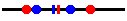
\includegraphics[width=100pt]{imgs/root_orderings_case4.png}
  & + & + & -
  \\ 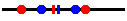
\includegraphics[width=100pt]{imgs/root_orderings_case5.png} & +
  & - & -
  \\ 
\includegraphics[width=100pt]{imgs/root_orderings_case8.png} & +
  & - & +
  \\ 
\includegraphics[width=100pt]{imgs/root_orderings_case2.png} & -
  & + & +
  \\ 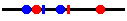
\includegraphics[width=100pt]{imgs/root_orderings_case3.png} & -
  & + & -
  \\ 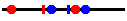
\includegraphics[width=100pt]{imgs/root_orderings_case6.png} & -
  & - & -
  \\ 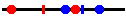
\includegraphics[width=100pt]{imgs/root_orderings_case7.png} & -
  & - & + \\ \hline
\end{tabular}

\noindent
We can compute the resultant sign exactly at 4 times the coefficient
precision.

\noindent
We can compute $\sign(C_R-C_B)$ exactly as $\sign(b_R a_B - b_B
a_R)\sign(a_R)\sign(a_B)$ at 2 times the coefficient precision.

\noindent
We can compute $\sign(P_R(C_B))$ exactly as $\sign(a_R b_B^2 - 2 b_R
a_B b_B + c_R a_B^2)$ at 3 times the coefficient precision.  The exact
sign is determined by the sign of $a_R$.\\

\noindent
For the case where $D_R=D_B$, we can do better by just computing
$\sign(C_R-C_B)$ and $\sign(D_R-4(C_R-C_B)^2)$ exactly at 4 times the
coefficient precision. These are sufficient to determine all of the
cases.\\

\noindent
For the case where $D_B=0$, we can do better by just computing
$\sign(C_R-C_B)$ and $\sign(D_R-(C_R-C_B)^2)$ exactly at 4 times the
coefficient precision. These are sufficient to determine all of the
cases.\\

\noindent
For the case where $D_B=D_R=0$, we can do better by just computing
$\sign(C_R-C_B)$ exactly at 2 times the coefficient precision. This is
sufficient to determine all of the cases.
\end{document}
